In this final step, we will analyze the design of an optimization algorithm combining the allocation of budget and the pricing when the seller a priori knows that every subcampaign is associated with a different context and charges a unique price to all the classes of users.

\subsubsection{Assumptions}
\begin{enumerate}
    \item The optimal bid is automatically set
    \item Single phase
\end{enumerate}

\subsubsection{Setup of the experiment}
For this experiment we will consider a time span $T=50$ days. Other variables are:
\begin{itemize}
    \item Total budget $b_{tot}$ that can be used for advertising
    \item The array of possible budgets $B$, e.g. the arms of the GPTS learners. (We used the same array for all learners)
    \item The array of possible prices $P$, e.g. the arms of the TS learners. (We used the same array for all learners)
    \item $C=3$ classes of users
    \item Maximum budget for each subcampaign: $b_{max_i}, 1 \leq i \leq C$ (the minimum is 0 for all subcampaigns)
    \item Minimum and maximum prices, that we set equal to 100 and 400.
    \item $\theta$ an array of 3 elements that contains the price pulled by the 3 TS learners on each day
    \item $d_p$ the estimation of the demand curve at price p provided by the TS learner
    \item $clicks$ is a $C \times |B|$ matrix, in which the element $i,j$ corresponds to the estimated number of clicks for the i-th ad with budget $B_j$
    \item $vpc$ is a $C \times |B|$ matrix, in which the element $i,j$ is the estimation of the value of one click on an ad of class i if the budget is set to $B_j$.
    \item $b_{best}$ is an array of size $C$ in which the i-th element represent the best budget allocation for class i
    \item $r_{exp}$ is an array of size $C$, the i-th element contains the expected revenue of class i
    \item $r_{max}$ the maximum among all the expected rewards
\end{itemize}

Also, we will have $C$ TS Learners to learn the best price, $C$ GPTS Learners to estimate the number of clicks as a function of the budget, and a CMAB optimizer to optimize the budget allocation among the subcampaigns.

\subsubsection{The algorithm}
The high-level pseudo code of the algorithm is shown in Algorithm \ref{alg:opt-constrained}.

Basically, every TS learner is responsible for finding the best price for the class of users it belongs to.
However, since only one price can be selected, the algorithm solves the budget optimization problem for each price and chooses the one that has the greatest expected reward.
In the budget optimization problem the value per click depends on the price chosen.
\begin{algorithm}
    \caption{Budget and Pricing optimization with fixed price}
    \label{alg:opt-constrained}
	\begin{algorithmic}[1]
        \FOR{$1 \leq t \leq T$}
        \STATE $\theta\gets ${draw a sample from all TS Learners}
        \FOR{$p \in \theta$}
        \STATE $d_p \gets demand(p)$
        \FOR{$1 \leq c \leq C$}
        \FOR{$1 \leq b \leq |B|$}
        \STATE $clicks_{c,b} \gets${Estimate clicks from GPTS learners}
        \STATE $vpc_{c,b}\gets${Estimate values per click}
        \ENDFOR
        \STATE $b_{best_c} \gets${Use CMAB optimizer to get best budget allocation}
        \STATE $r_{exp_i} \gets${Use CMAB optimizer to get expected revenues}
        \ENDFOR
        \ENDFOR
        \STATE $r_{max} \gets \max{r_{exp_i}}$
        \STATE $(\bar{p}, \bar{b_c}) \gets${Select best price and budgets associated with best revenue}
        \STATE $(\bar{c}, \bar{b}, \bar{r}) \gets${Test with env and get real clicks, buys and revenue}
        \STATE Update TS and GPTS learners
        \ENDFOR
	\end{algorithmic}
\end{algorithm}
\newpage Some remarks:
\begin{itemize}
    \item All the TS learners have 6 arms. As discussed in \ref{pricing_best_arm}, this guarantees a fair reward with the given timespan. 
    \item The value $d_p$ is estimated from the TS learner, in particular it returns a sample from the beta distribution of price $p$, in the following way: $d_p = beta(\alpha_p, \beta_p)$
    \item To estimate the clicks given a class $c$ and a budget $b$, the c-th GPTS learner returns a sample from the normal distribution of budget $b$, in which mean and variance are learned by the GP regressor.
    \item the estimation of the values per click is obtained with the following formula: 
    \[ vpc_{c,b} = \frac{p * clicks_{c,b} * d_p - B_b}{clicks_{c,b}} \;\; \forall c \in \{1,..,C\} \; \forall b \in \{1,..,|B|\} \]
    in which the numerator represents the net expected revenue (net revenue - budget spent), and is divided by the expected number of clicks to obtain the values per click, for each class and for each budget.
    \item The CMAB optimizer takes as input the estimated values per clicks and number of clicks of each subcampaign and returns the best budget allocation by solving the knapsack problem.
    \item In the final part the TS and GPTS learners are updated. In particular, the c-th GPTS takes the number of clicks that the c-th subcampaign received and uses them to update the model on its pulled arm.
    Instead, each TS learner is updated on the same arm $\bar{p}$ but with different inputs: the c-th TS learner updates its arm $\bar{p}$ with the number of buys $\bar{b_c}$ that come from the c-th subcampaign as successes, and $\bar{c_c} - \bar{b_c}$ as the number of failures
\end{itemize}

\subsubsection{Results}
After running the algorithm for 50 days with 1000 experiments, we obtained the regret shown in figure \ref{fig:opt_constrained_regret}.
As in the previous points, this regret refers to the best arms, and it represents how fast the algorithm converges to the best solution.

\begin{figure}
    \caption{Cumulative regret}
    \label{fig:opt_constrained_regret}
    \makebox[\textwidth][c]{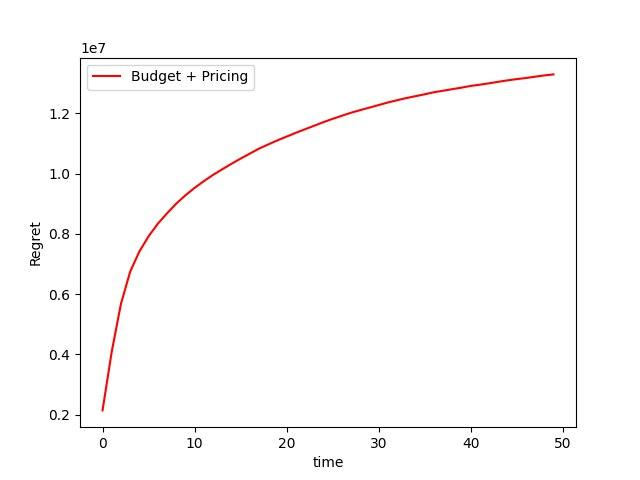
\includegraphics[width=0.80\textwidth]{sections/images/opt_constrained_regret.jpg}}
\end{figure}

\begin{figure}
    \caption{Reward}
    \label{fig:opt_constrained_reward}
    \makebox[\textwidth][c]{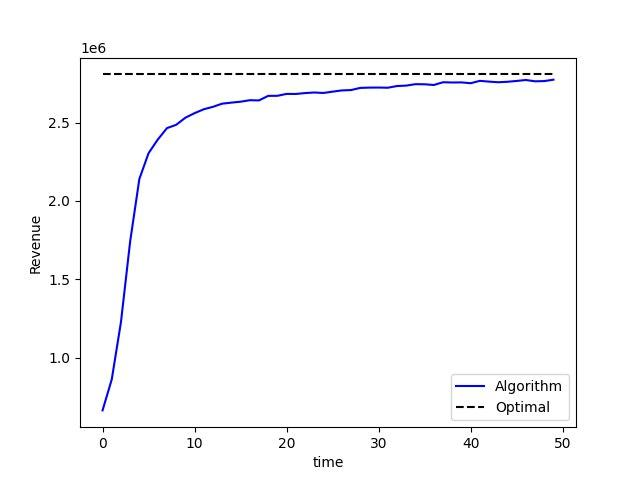
\includegraphics[width=0.80\textwidth]{sections/images/opt_constrained_reward.jpg}}
\end{figure}